\documentclass[a4paper]{scrartcl}
%\documentclass[a4paper, 10pt]{scrartcl}
\usepackage[czech]{babel}
\usepackage[utf8]{inputenc}
\usepackage{a4wide}

\usepackage{graphicx}


\title{Význam osobního managementu pro můj osobní rozvoj}
\subtitle{}
\author{Iveta Terezie Pelikánová}
\date{}

\begin{document}
\maketitle 

\noindent
Tento týden jsem shodou všech náhod dočetla knihu Sebekoučink pro ženy od německé koučky Cornelie Topf \cite{topf2014}. Nebylo to poprvé, co jsem se pokusila 
tuto knihu přečíst, již dlouhou dobu mi ležela v knihovně od prvního pokusu prokousat se jejím obsahem. Kniha není dlouhá, její druhé čtení mi nezabralo ani celý 
týden, ale když jsem ji otevřela asi před dvěma roky poprvé, nějak jsem necítila její kouzlo ani pocit, že by mi informace v ní v životě k něčemu byly, resp. že 
bych je byla schopna aplikovat. A právě tuto moji niternou proměnu, bych přiřadila osobnímu rozvoji. Když se teď po dlouhé době opět vracím k osobnostním 
charakteristikám při studiu na Masarykově ústavu vyšších studií, udivuje mě, že jsem se až do tohoto okamžiku dostala. Občas mě taky překvapí, že ještě žiji - se 
svou snad ještě labilnější melancholií než na střední škole\cite{odmaturuj2004}. Můj život velmi dobře popisují sbírky komiksů mladé kreslířky z Brooklynu Sarah 
Andersenové - Dospělost je mýtus a Ubulená hromádka štěstí \cite{dospelost_je_mytus,hromada_stesti}.
    
    \begin{figure}[h]
        \centering
        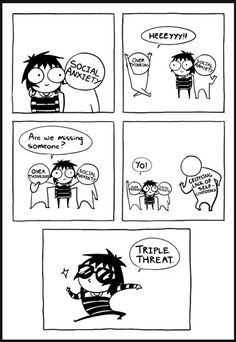
\includegraphics[width=0.44\textwidth]{triple_threat.jpg}
        \caption{Moje trojka.\cite{hromada_stesti}}
    \end{figure}

Velmi doporučuji, nikdy bych neřekla, že něco dokáže tak dokonale vystihnout, jak se cítím, co mi moje id podsouvá a jaký vedu svůj vnitřní dialog.\\

\indent Jsem extrémně skeptická ke školením self managementu a knihám o osobním rozvoji. Nikdy bych si nedovolila někomu prodávat svoje zaručené know-how, jak 
být lepší, neprokrastinovat a být efektivnější. Když Petr Ludwig napsal svoji knihu Konec prokrastinace \cite{ludwig2013} dostala se mi do ruky a já s velkým 
očekáváním ji velmi rychle přečetla - přece jen obsahuje velké množství obrázků. Myslím, že jde o velmi dobrou průvodní knihu a že z ní každý člověk může čerpat 
něco, co bude vyhovovat právě jemu. Ale nikdy není něco vhodné pro všechny. Pamatuji si, když měl Petr první přednášku na ČVUT, v době kdy se jeho byznys 
poradenství teprve rodil, byla beznadějně obsazená. Měla jsem jeho knihu přečtenou a chtěla jsem něco víc. Nepřipadalo mi, že bych mohla z knihy něco praktikovat 
- vlastně jsem neměla problém s prokrastinací, ale chtěla jsem být efektivnější. Přednáška byla velmi hezká, všichni hltali jeho slova a dělali si poznámky. Na 
závěr několik lidí vyzval, aby se s ostatními podělili o to, co se jim líbilo případně nelíbilo a co si odnáší domů. Zpětná vazba byla bez zaváhání pozitivní. 
Nevím, jestli v té posluchárně někdo sdílel moje pocity, které byly úplně odlišné. Byla jsem vytočená a naštvaná, protože neřekl ani o slovo víc, než bylo 
napsané v knize. Byla jsem zklamaná. Uvažovala jsem, že mu to půjdu říct, slušně poděkovat za přednášku, protože byla kvalitní, ale dát mu zpětnou vazbu, že jako 
čtenář jeho knihy mi ta přednáška nic nepřinesla. Nakonec jsem se rozhodla svoje pocity přejít, hlavně protože kolem Petra byla pořád fronta lidí, a jít domů. 
Když jsem za 20 minut čekala na peróně metra, všimla jsem si, že tam Petr Ludwig stojí s kolegou. Zamyslela jsem se a sebrala veškerou odvahu, kterou jsem měla a 
šla jsem si s ním promluvit o jeho přednášce. Cítila jsem zodpovědnost, aby měl plnohodnotnou zpětnou vazbu a ne jen pozitivní ohlasy. Vysvětlila jsem mu svoje 
rozčarování, poděkovala mu a on vzal kritiku velmi dobře. Tato zkušenost mě posunula ohromně vpřed - překonala jsem svůj strach a odstup a dokázala jsem podat 
konstruktivní kritiku cizímu člověku. Byla jsem na sebe hrdá, ale stála jsem před novou výzvou. Konec prokrastinace není vhodná kniha pro mě, tak jak být lepší? 
\\

\indent Během dalších let jsem studovala knihy jako Zen To Done \cite{babauta2009} od Lea Babauta nebo Vzdělávejte se po svém: nechte přednášek, ušetřete spoustu 
peněz a naučte se víc, než se kdy naučí vaši vrstevníci \cite{stephens2013} od Dalea J. Stephense. Občas jsem si pustila video z konferencí TED nebo TEDx 
\cite{ted}. A celou tu dobu jsem měla pocit, že nejsem dost dobrá, že toho dělám málo. Že nepatřím na vysokou školu, že mý spolužáci jsou mnohem chytřejší, mají 
lepší známky, víc se té škole věnují. Já jsem při studiu jaderné chemie vedla studentské Audiovizuální studiu Silicon Hill, technicky i lidsky jsem produkovala 
menší i větší akce třeba z Václavského náměstí a v neziskovém centru, kde všichni pracují bez nároku na honorář, se mi za rok podařilo vydělat víc jak 500 tisíc 
Kč (dřív to bylo tak maximálně 200 tisíc Kč). Ale pro mě to bylo málo. Nevadilo mi, že Ibalgin beru téměř každý den ve dvojnásobném doporučeném dávkování, aby mě
nebolely záda ze stresu, neměla jsem čas přemýšlet o sobě samé, měla jsem zodpovědnost za projekty a ostatní lidi, očekávali se ode mě dobré výsledky a 
spolehlivost, nebo alespoň já jsem to očekávala. Byla to dlouhá cesta k sebepoznání a sebepřijetí. Přesvědčit sebe sama, že nemusím skončit v nemocnici na 
kapačkách, abych si mohla odpočinout. Že smyslem mého života není pomoci všem a zachránit svět, že jsem zodpovědná za sebe sama a když sebudu cítit dobře, že i 
lidé kolem mne se budou cítit dobře. Nemusím udělat mnoho, třeba jen obyčejný úsměv může někomu změnit celý den. Po malých krůčkách sebepřijetí bez žádného 
zázračného návodu. S mužem, který místo aby mě bezmezně podpořil mi upřímně sdělil často velmi bolestivou pravdu, kterou jsem asi nechtěla slyšet. Ale svým 
příkladem mě naučil občas odpočívat, dokázat říci ne a občas dát přednost sebe sama před světem. \\

\indent Před rokem touto dobou jsem byla ještě rozhodnutá, že dokončím v červnu 2018 magisterské studium a půjdu někam pracovat. Nedokázala jsem si představit, 
že budu dělat vědu. Ale myslím si, že právě díky osobnímu managementu jsem právě teď tam, kde jsem. Vím, že kdybych svoje vysokoškolské studium víc soustředila 
na školu, bylo by to teď o něco jednodušší - nedostudovávala bych spoustu věcí. Na druhou stranu bych neměla nadhled a zkušenosti s vedením týmu a nevěděla bych, 
jak funguje komerční velký svět. Ujasnila jsem si své cíle a kde jsou moje limity. Chtěla bych být máma velké rodiny a nestojím o rozjezd velké kariéry, kterou 
pak budu muset opustit kvůli dětem. Proto mi teď práce v laboratoři a doktorské studium dává dobrý smysl. Pedagogika a univerzita mi také přijde jako vhodné 
prostředí pro částečné úvazky. A třeba se mi někdy splní i můj sen být paní docentka a být příkladem, že když člověk chce jít za svými sny, tak se mu splní. 
Prostě že i v oboru jaderné chemii mohou existovat docentky a ne jen docenti a profesoři.\\


\indent Může to trochu znít, že jsem stabilní, vyzrálá osobnost, ale skutečnost je trochu jiná. Boj s vlastním perfekcionismem a se srovnáním s ostatními lidmi 
jsem ještě úplně nevyhrála, to je cesta mého osobního rozvoje. Každý den se učit být spokojená tam kde jsem, dělat maximum pro druhé ale i sebe. Snažit se 
vybalancovat čas v práci a čas s partnerem. Naučit se asertivně komunikovat a nebát se říct své názory. Umět si je obhájit a zpochybňovat je. Naučit se rychle a 
pohotově reagovat a umět odhadnout komunikaci. Jak mi to půjde a jaké k tomu použiji metody či pomůcky netuším, ale co vím jistě je, že mi v tom žádný kurz ani 
kniha nedá univerzální návod. Já jsem jiná, možná úplně obyčejná, mám svoji historii, psychologický vývoj svojí osobnosti, který předurčuje, jak zpracovávám 
informace, co dokážu přijmout a jaká forma mi prostě vyhovuje. Každý si musíme najít svoji vlastní cestu. \\

\indent 
Mám velmi špatnou paměť, značně selektivní a silně spjatou s emocemi, proto používám Google Calendar \cite{calendar}, kam si píšu schůzky, předměty, společenské 
akce, vše s konkrétními časy a místy, kam dorazit. Vždycky, když přijdu pozdě někam výuku, tak jsem si to špatně poznamenala nebo špatně přečetla. V práci 
používám ještě papírový kalendář, kde si poznamenávám pouze hesla, abych přehledně viděla, co se bude dít. Mimo to v online kalendáři vidím akce, jiných lidí - 
audiovizuálního centra, své drahé polovičky, takže si mohu vybrat, komu mohu případně pomoci a jak vše dobře sesynchronizovat. Většinu úkolů si poznamenávám do 
aplikace ToDoIst \cite{todoist} - včetně data, kdy má být úkol splněn, protože pamatovat si úlohy je pro mě nemyslitelné. Pro různé oblasti mám vytvořené složky, 
kde shromažďuji úkoly k jednomu tématu: práce, druhá práce, domácí práce, MUVS, nákupní seznam, groceries. Každý splněný úkol mě potěší a zaznamenávání věcí jako 
konkrétní úkoly, které jsou splnitelné je pro mě samozřejmostí. Nepoužívám například "uklidit kuchyni", ale konkrétně "vynést koš", "umýt sporák" a další. 
Krátkodobé čí náhlé úkoly si často poznamenávám na malé nalepovací papírky, které polepuji po notebooku či monitoru, abych na něco nezapomněla. Při práci v 
laboratoři používám nejčastěji laboratorní deník - klasický papírový. Píšu si do něj každý den a zmiňuji nejen práci v laboratoři, ale také aktivity mimo 
laboratoř, abych později věděla, proč nemám v daný čas uvedenou nějakou konkrétní práci, protože jsem například byla na konzultaci k předmětu nebo protože jsem 
natáčela někde seminář, či jsem jen měla schůzku. Mnohem lépe se mi potom reportuje, co jsem již zvládla udělat. Nemám potom pocit, že jsem nějaký čas 
promarnila, protože například zjistím, že jsem dva dny moc práce neudělala, ale opravila jsem protokoly studentům do Praktického cvičení nebo jsem se věnovala 
vědecké rešerši na určité téma.\\

Z výuky, kterou ještě absolvuji nebo z odborných článků, které čtu jsem se snažila si taky dělat poznámky na papír, ale velmi špatně se mi četly a také 
udržovaly na jednom místě. Od podzimu si, pokud to jen trochu jde, dělám poznámky do textového souboru v počítači (klasický textový soubor .tex, ale s příponou 
.md), který mám nastavený na formátování markdown - umožňuje text zobrazit se základním formátováním - tučné písmo či kurzíva, nebo vložit obrázky. O svoji 
práci mám trochu strach a tak používám verzovací systém git a verzuji sobory na Github \cite{github} nebo Gitlab \cite{gitlab}, který také umí textové soubory s 
formátováním markdown zobrazit, takže se k poznámkám dostanu odkudkoliv a i z telefonu. Samozřejmě občas vše zálohuji na další externí medium mimo počítač.\\

\indent Čím tuto úvahu zakončit? Než jsem se do psaní pustila dívala jsem se na odborné články, které obsahují jako klíčové slovo self-management. Překvapilo 
mě, že za posledních deset let každý rok vyjde v průměru 28 000 takových článků. Z čeho jsem byla ještě více překvapená, že nejčastěji jde o self-management u 
pacientů s onkologickým onemocněním či diabetem 2. typu nikoliv self-management pracujících lidí. Narazila jsem také na články o kompetencích učitelů a studentů 
vysoké školy a také o self-managementu studentů dálkového studia. Bohužel se nakonec tato témata nehodila do mého konceptu této eseje, ale chystám se tyto 
články prostudovat. Ráda se opět vrátím v několika publikacích k osobnímu rozvoji, ale doufám, že už nikdy nezapomenu, že mojí cestou nikdo jiný kráčet nemůže a 
ani nekráčel a s tímto vědomím budu přistupovat k svému osobnímu rozvoji, svojí práci i svému osobnímu životu.\\


\vspace{36pt}
\indent Tento text byl vypracován k udělení zápočtu z předmětu {\it Self management učitele}.

\bibliographystyle{unsrt} % We choose the "plain" reference style
\bibliography{literatura} % Entries are in the "refs.bib" file

\end{document}